%==============================================================================%
%================================== intro =====================================%
\section{Introduction}
\subsection{LBGB au sein du Genoscope et du CEA}
Le Genoscope (CNS\footnote{Centre National de Séquençage}) a été créé en 1996 pour participer au projet mondial de séquençage du génome humain (\emph{Human Genome Project}) qui à débuté en 1988 et c'est terminé en 2007, notament dans l'objectif de séquencer le chromosomes 14 humain. Lors de sa cration le genoscope à égalment été missioné de développer de programme de génomique en france dans le cadre du projet France génomique. Le laboratoire de bioinformatique pour la génomique et la biodiversité (\textbf{LBGB}) fait partie du genoscope qui est une direction de l'institut François Jacob (Jacob) de la direction de la recherche fondamental (\textbf{DRF}) du Commissariat à l'énergie atomique et aux énergies (\textbf{CEA}), comme on peut l'observé sur l'organigramme de la figure \ref{organigramme_LBGB} qui situe la laboratoire au sein du genoscope et de CEA.

\begin{figure}[H]
    \centering
    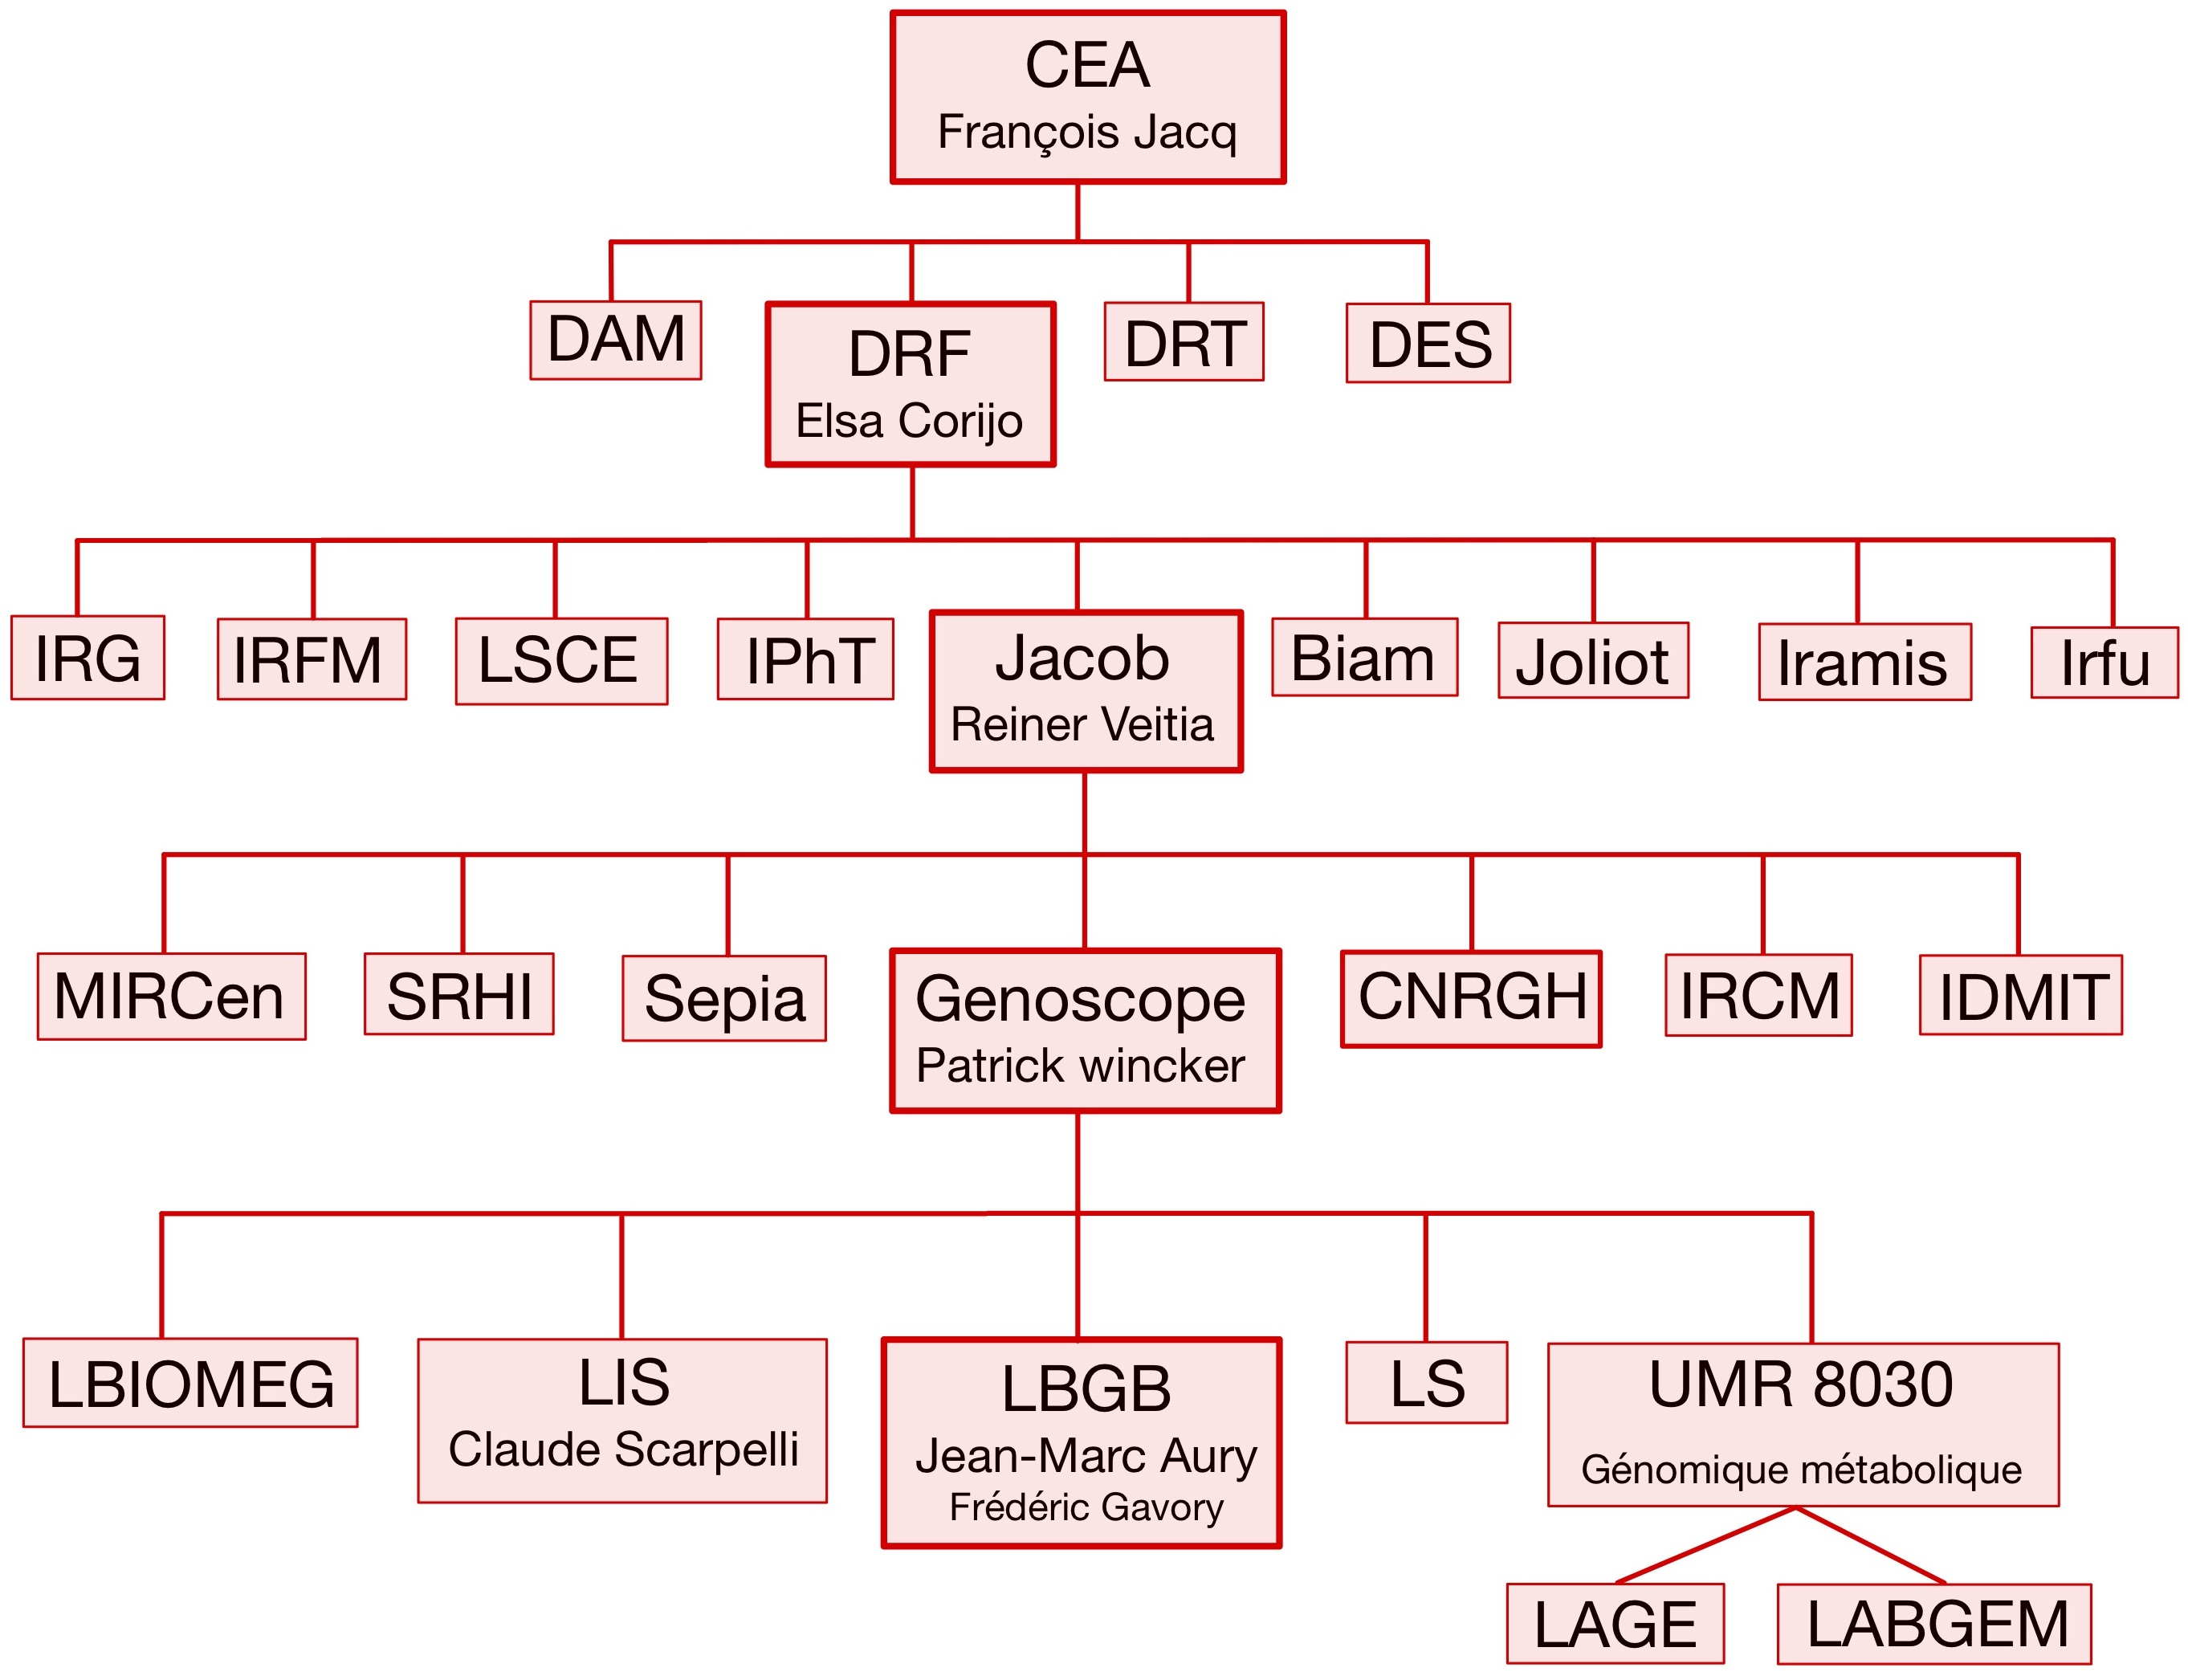
\includegraphics[width=1\textwidth]{img/organigramme.jpg}
    \caption{Organigramme situant l’équipe du Laboratoire de Bioinformatique pour la Génomique et la Biodiversité (LBGB) au sein du genoscope et du CEA}
    \label{organigramme_LBGB}
\end{figure}
%==============================================================================%
%=============================== Objectifs ====================================%
\section{Ojectifs}

%==============================================================================%
%================================ Méthodes ====================================%
\section{Méthodes}

%==============================================================================%
%================================ Resultats ===================================%
\section{1$^{\text{er}}$ Résultats}

%==============================================================================%
%======================== Conclusion et perspectives ==========================%
\section{Conclusion et Perspectives}
